
%(BEGIN_QUESTION)
% Copyright 2007, Tony R. Kuphaldt, released under the Creative Commons Attribution License (v 1.0)
% This means you may do almost anything with this work of mine, so long as you give me proper credit

Tegn responsen til en regulator med {\it kun integralvirkning}, med integralkonstant 1 minutt per repetisjon, for følgende inngangsbetingelser. Anta at regulatoren er {\it direktevirkende}:

$$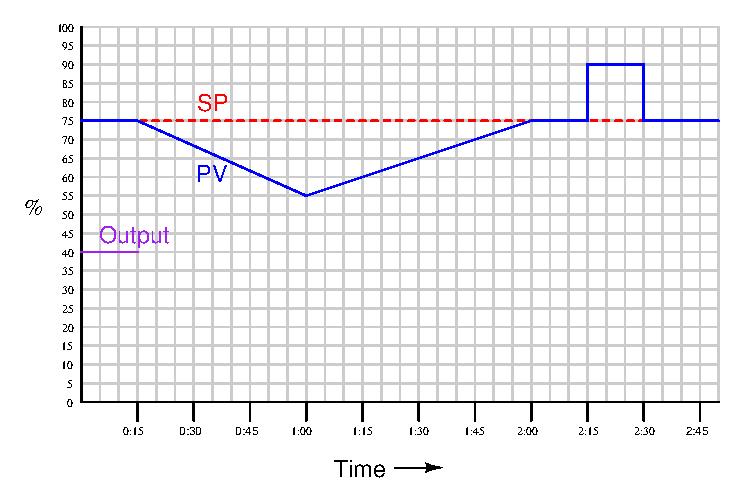
\includegraphics[width=15.5cm]{i01605x01.eps}$$

Tidsskalaen i diagrammet er minutter:sekunder, og I-only algoritmen er som følger:

$$m = {1 \over \tau_i} \int e \> dt$$

\noindent
Der,

$m$ = regulatorutgang (manipulert variabel)

$e$ = avvikssignal (PV$-$SP)

$\tau_i$ = integraltidskonstant

\vskip 10pt

\underbar{file i01605}
%(END_QUESTION)





%(BEGIN_ANSWER)

$$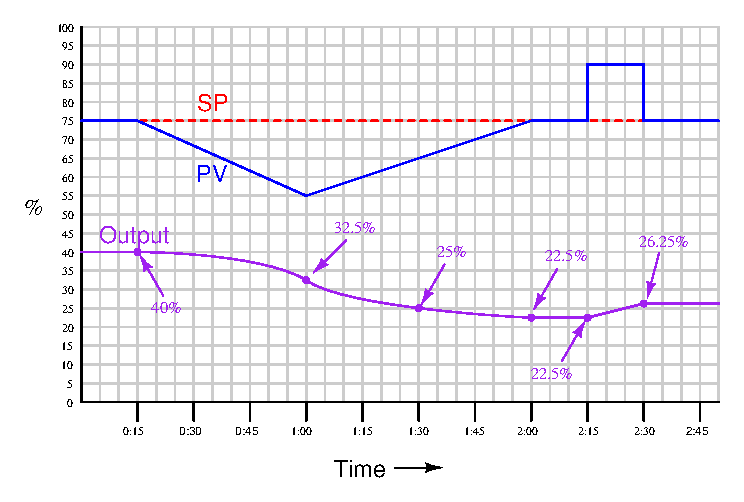
\includegraphics[width=15.5cm]{i01605x02.eps}$$

Når integralvirkningen beregnes i første fase av PV-avviket fra SP: arealet akkumulert under kurven mellom 0:15 og 1:00 er 7.5 \%-min (7.5 ``prosent-minutter,'' som er produktet av prosentavvik og tid i minutter). Siden regulatoren har tenkt forsterkning lik 1 og integralkonstant 1 minutt per repetisjon (eller 1 repetisjon per minutt), blir 100\% av denne akkumuleringen bidrag til utgangen, og den drives ned fra 40\% til 32.5\%. Utgangssignalet går ned sammen med negativt avvik (PV $-$ SP), fordi dette er en direktevirkende regulator:
 
$$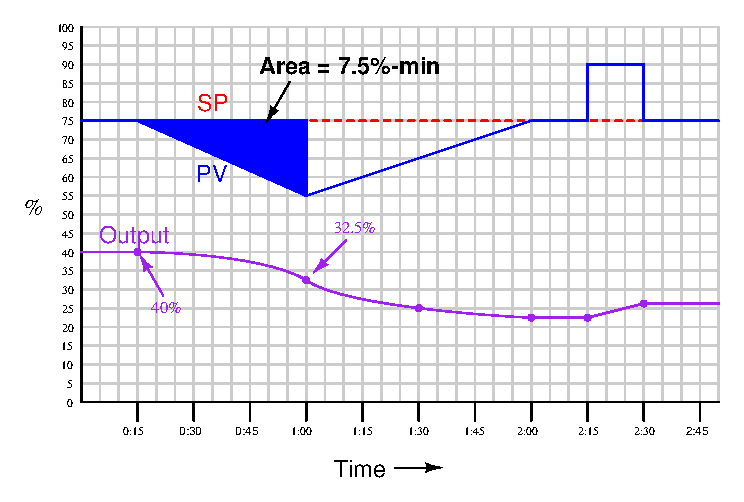
\includegraphics[width=15.5cm]{i01605x03.eps}$$

I neste fase av PV-avviket er akkumulert trekantareal 10\%-min (en trekant med høyde 20\% og lengde 1 minutt). Dette driver regulatorutgangen ytterligere 10\% ned ved tid = 2:00, fra 32.5\% til 22.5\%.
 
$$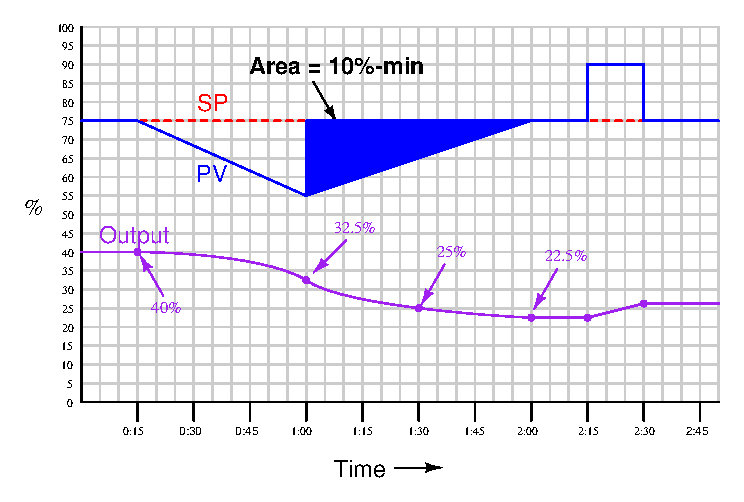
\includegraphics[width=15.5cm]{i01605x04.eps}$$

Etter at PV har returnert til SP, gir integralvirkningen ingen videre endring i utgangen. Deretter, mellom 2:15 og 2:30, gir avviket på 15\% i 15 sekunder (0.25 minutter) en avvik-tid akkumulering på 3.75 \%-min, og dette legges til utgangssignalet slik at vi ender med 26.25\% utgang når PV returnerer til SP:
 
$$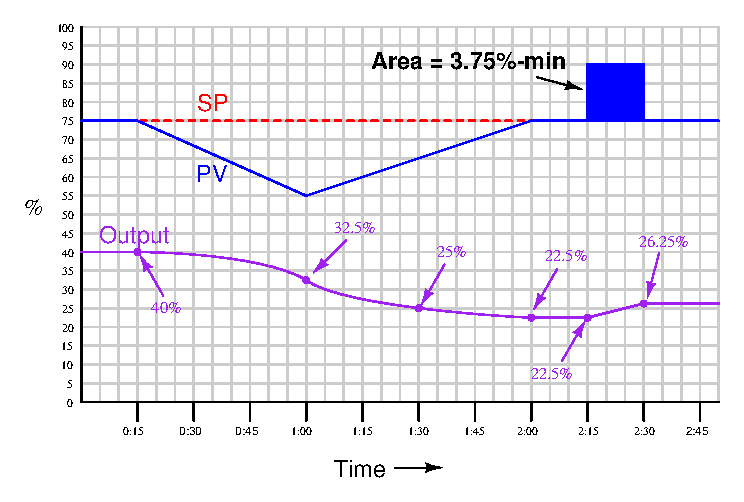
\includegraphics[width=15.5cm]{i01605x05.eps}$$

Merk hvordan integralvirkningen får utgangen til å rampe med variabel hastighet mellom 0:15 og 1:00, og igjen mellom 1:00 og 2:00. Mellom 2:15 og 2:30 gir integralvirkningen derimot lineær stigning, på grunn av det rektangulære avviket i dette tidsrommet.

%(END_ANSWER)





%(BEGIN_NOTES)


%INDEX% Control, integral: graphing controller response

%(END_NOTES)
